\PassOptionsToPackage{unicode=true}{hyperref} % options for packages loaded elsewhere
\PassOptionsToPackage{hyphens}{url}
%
\documentclass[]{book}
\usepackage{lmodern}
\usepackage{amssymb,amsmath}
\usepackage{ifxetex,ifluatex}
\usepackage{fixltx2e} % provides \textsubscript
\ifnum 0\ifxetex 1\fi\ifluatex 1\fi=0 % if pdftex
  \usepackage[T1]{fontenc}
  \usepackage[utf8]{inputenc}
  \usepackage{textcomp} % provides euro and other symbols
\else % if luatex or xelatex
  \usepackage{unicode-math}
  \defaultfontfeatures{Ligatures=TeX,Scale=MatchLowercase}
\fi
% use upquote if available, for straight quotes in verbatim environments
\IfFileExists{upquote.sty}{\usepackage{upquote}}{}
% use microtype if available
\IfFileExists{microtype.sty}{%
\usepackage[]{microtype}
\UseMicrotypeSet[protrusion]{basicmath} % disable protrusion for tt fonts
}{}
\IfFileExists{parskip.sty}{%
\usepackage{parskip}
}{% else
\setlength{\parindent}{0pt}
\setlength{\parskip}{6pt plus 2pt minus 1pt}
}
\usepackage{hyperref}
\hypersetup{
            pdftitle={Power-Electronic Control Handbook},
            pdfauthor={Flemming Abrahamsen},
            pdfborder={0 0 0},
            breaklinks=true}
\urlstyle{same}  % don't use monospace font for urls
\usepackage{longtable,booktabs}
% Fix footnotes in tables (requires footnote package)
\IfFileExists{footnote.sty}{\usepackage{footnote}\makesavenoteenv{longtable}}{}
\usepackage{graphicx,grffile}
\makeatletter
\def\maxwidth{\ifdim\Gin@nat@width>\linewidth\linewidth\else\Gin@nat@width\fi}
\def\maxheight{\ifdim\Gin@nat@height>\textheight\textheight\else\Gin@nat@height\fi}
\makeatother
% Scale images if necessary, so that they will not overflow the page
% margins by default, and it is still possible to overwrite the defaults
% using explicit options in \includegraphics[width, height, ...]{}
\setkeys{Gin}{width=\maxwidth,height=\maxheight,keepaspectratio}
\setlength{\emergencystretch}{3em}  % prevent overfull lines
\providecommand{\tightlist}{%
  \setlength{\itemsep}{0pt}\setlength{\parskip}{0pt}}
\setcounter{secnumdepth}{5}
% Redefines (sub)paragraphs to behave more like sections
\ifx\paragraph\undefined\else
\let\oldparagraph\paragraph
\renewcommand{\paragraph}[1]{\oldparagraph{#1}\mbox{}}
\fi
\ifx\subparagraph\undefined\else
\let\oldsubparagraph\subparagraph
\renewcommand{\subparagraph}[1]{\oldsubparagraph{#1}\mbox{}}
\fi

% set default figure placement to htbp
\makeatletter
\def\fps@figure{htbp}
\makeatother

\usepackage{booktabs}
\usepackage[]{natbib}
\bibliographystyle{apalike}

\title{Power-Electronic Control Handbook}
\author{Flemming Abrahamsen}
\date{2023-02-18}

\begin{document}
\maketitle

{
\setcounter{tocdepth}{1}
\tableofcontents
}
\hypertarget{preface}{%
\chapter{Preface}\label{preface}}

This is a collection of technical notes centered around control of power electronics and drives.

\hypertarget{transformations}{%
\chapter{Transformations}\label{transformations}}

\hypertarget{vector-definition}{%
\section{Vector definition}\label{vector-definition}}

\[
\begin{aligned}
\underline{v} 
& = \frac{2}{3} \left( v_a + v_b e^{j \frac{2 \pi}{3}}+ v_c e^{j \frac{4 \pi}{3}} \right)\\
& = \frac{2}{3} \left( v_a + v_b (- \frac{1}{2}+j\frac{\sqrt{3}}{2}) + v_c (- \frac{1}{2}-j\frac{\sqrt{3}}{2}) \right)\\
& = \left(\frac{2}{3} v_a - \frac{1}{3}  (v_b+v_c) \right) + j \left( \frac{1}{\sqrt{3}} (v_b-v_c) \right)   \\
& = \frac{2}{3} \left( v_a - \frac{1}{2}  (v_b+v_c) \right) + j \frac{2}{3} \left( \frac{\sqrt{3}}{2} (v_b-v_c) \right)   \\
& = v_\alpha + j v_\beta   \\
\end{aligned}
\label{eq:trans1}
\]
\#\#\# Vector amplitude

\[
|\underline{v}| = \sqrt{v_\alpha^2 +  v_\beta^2}
\label{eq:trans1a}
\]

\hypertarget{abc-to-alpha-beta}{%
\section{abc to alpha-beta}\label{abc-to-alpha-beta}}

System with a zero-component:

\[
\begin{bmatrix} \alpha\\ \beta \\ 0 \end{bmatrix}
= \begin{bmatrix} \frac{2}{3} & -\frac{1}{3} & -\frac{1}{3} \\ 0 & \frac{1}{\sqrt{3}} & -\frac{1}{\sqrt{3}} \\ \frac{1}{3} & \frac{1}{3} & \frac{1}{3} \end{bmatrix}
\begin{bmatrix} a\\ b \\ c \end{bmatrix}
= \frac{2}{3} \begin{bmatrix} 1 & -\frac{1}{2} & -\frac{1}{2} \\ 0 & \frac{\sqrt{3}}{2} & -\frac{\sqrt{3}}{2} \\ \frac{1}{2} & \frac{1}{2} & \frac{1}{2} \end{bmatrix}
\begin{bmatrix} a\\ b \\ c \end{bmatrix}
\label{eq:trans3}
\]

\[
\begin{aligned}
\alpha &= \frac{2}{3}(a - \frac{1}{2}(b+c)) \\
\beta &= \frac{1}{\sqrt{3}}(b-c) \\
0 &= \frac{1}{3}(a+b+c)
\end{aligned}
\label{eq:trans1}
\]

\[
\begin{bmatrix} \alpha\\ \beta \end{bmatrix}
= \begin{bmatrix} \frac{2}{3} & -\frac{1}{3} & -\frac{1}{3} \\ 0 & \frac{1}{\sqrt{3}} & -\frac{1}{\sqrt{3}} \end{bmatrix}
\begin{bmatrix} a\\ b \\ c \end{bmatrix}
= \frac{2}{3} \begin{bmatrix} 1 & -\frac{1}{2} & -\frac{1}{2} \\ 0 & \frac{\sqrt{3}}{2} & -\frac{\sqrt{3}}{2} \end{bmatrix}
\begin{bmatrix} a\\ b \\ c \end{bmatrix}
\label{eq:trans2}
\]

\[
\begin{bmatrix} a\\ b \\ c \end{bmatrix}
= \begin{bmatrix} 1 & 0 & 1 \\ -\frac{1}{2} & \frac{\sqrt{3}}{2} & 1 \\ -\frac{1}{2} & -\frac{\sqrt{3}}{2} & 1 \end{bmatrix}
\begin{bmatrix} \alpha\\ \beta \\ 0 \end{bmatrix}
\label{eq:trans4}
\]

\hypertarget{modulation}{%
\chapter{Modulation}\label{modulation}}

The modulation described here is based on space-vectors.

\hypertarget{two-level-space-vectors}{%
\section{Two-Level Space Vectors}\label{two-level-space-vectors}}

Two-level modulation has six active vectors and two zero-vectors. Each vector is calculated from the general voltage vector formula as here below. The voltage vector subscript denotes the switch level for phases a, b and c, where 1 means the voltage is clamped to high rail of the dc-link voltage and 0 means the voltage is clamped to the low rail.

\[
\begin{aligned}
\underline{v}_{100} 
& = \frac{2}{3} \left( \frac{V_d}{2} - \frac{V_d}{2} e^{j \frac{2 \pi}{3}}- \frac{V_d}{2} e^{j \frac{4 \pi}{3}} \right)\\
& = \frac{2}{3} \frac{V_d}{2} \left( 1-  (- \frac{1}{2}+j\frac{\sqrt{3}}{2}) - (- \frac{1}{2}-j\frac{\sqrt{3}}{2}) \right)\\
& = \frac{2}{3} \frac{V_d}{2} 2\\
& = \frac{2}{3} V_d\\
\end{aligned}
\]

\begin{figure}
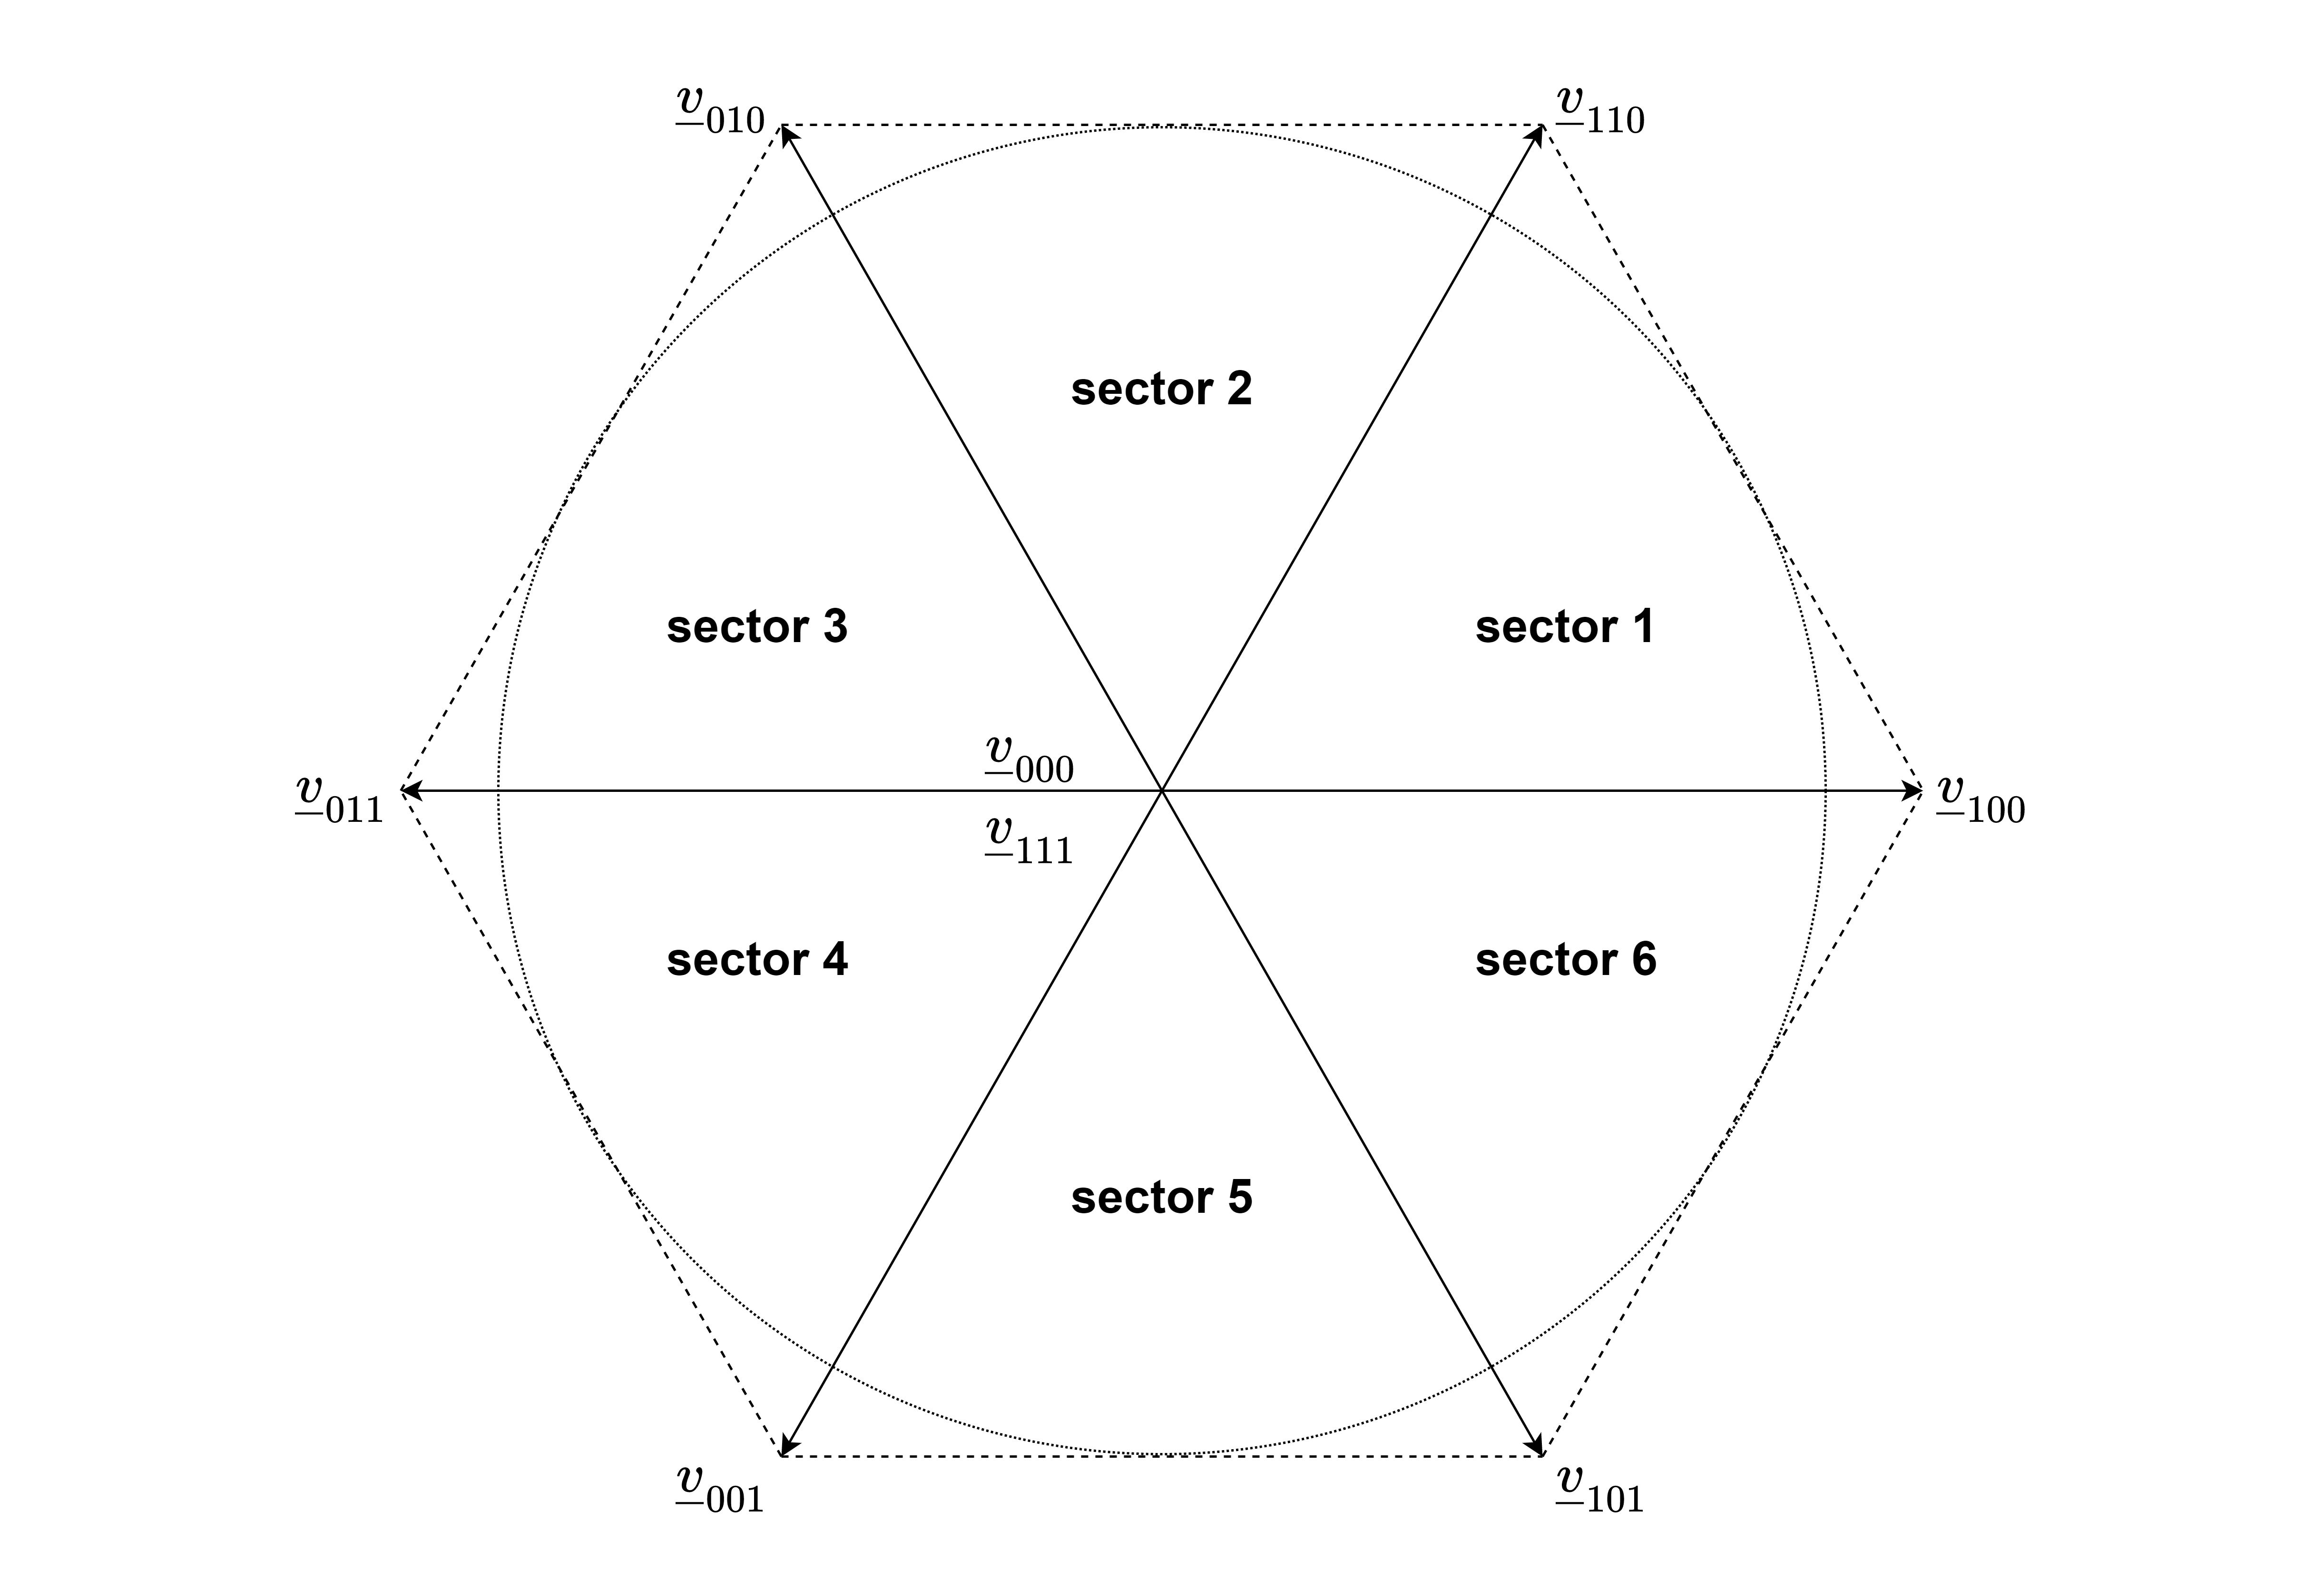
\includegraphics[width=1\linewidth]{images/modulation/hexagon} \caption{Hexagon with the six active vectors and two zero vector.}\label{fig:unnamed-chunk-1}
\end{figure}

Similarly, all the vectors are derived as:

\[
\begin{aligned}
\underline{v}_{000} &  = 0\\
\underline{v}_{100} &  = \frac{2}{3} V_d\\
\underline{v}_{110} &  = \frac{2}{3} V_d (\frac{1}{2}+j\frac{\sqrt{3}}{2})\\
\underline{v}_{010} &  = \frac{2}{3} V_d (-\frac{1}{2}+j\frac{\sqrt{3}}{2})\\
\underline{v}_{011} &  = -\frac{2}{3} V_d\\
\underline{v}_{001} &  = \frac{2}{3} V_d (-\frac{1}{2}-j\frac{\sqrt{3}}{2})\\
\underline{v}_{101} &  = \frac{2}{3} V_d (\frac{1}{2}-j\frac{\sqrt{3}}{2})\\
\underline{v}_{111} &  = 0\\
\end{aligned}
\]

\hypertarget{calculation-of-duty-cycles.}{%
\section{Calculation of duty-cycles.}\label{calculation-of-duty-cycles.}}

It is possible realize a voltage vector anywhere inside the hexagon on the figure above. Any reference voltage will be located in one of the six sectors, and as it generally desired to avoid unnecessary switching, the reference vector will be realized with the two neighboring active vectors and zero-vectors by geometrical considerations.

\begin{figure}
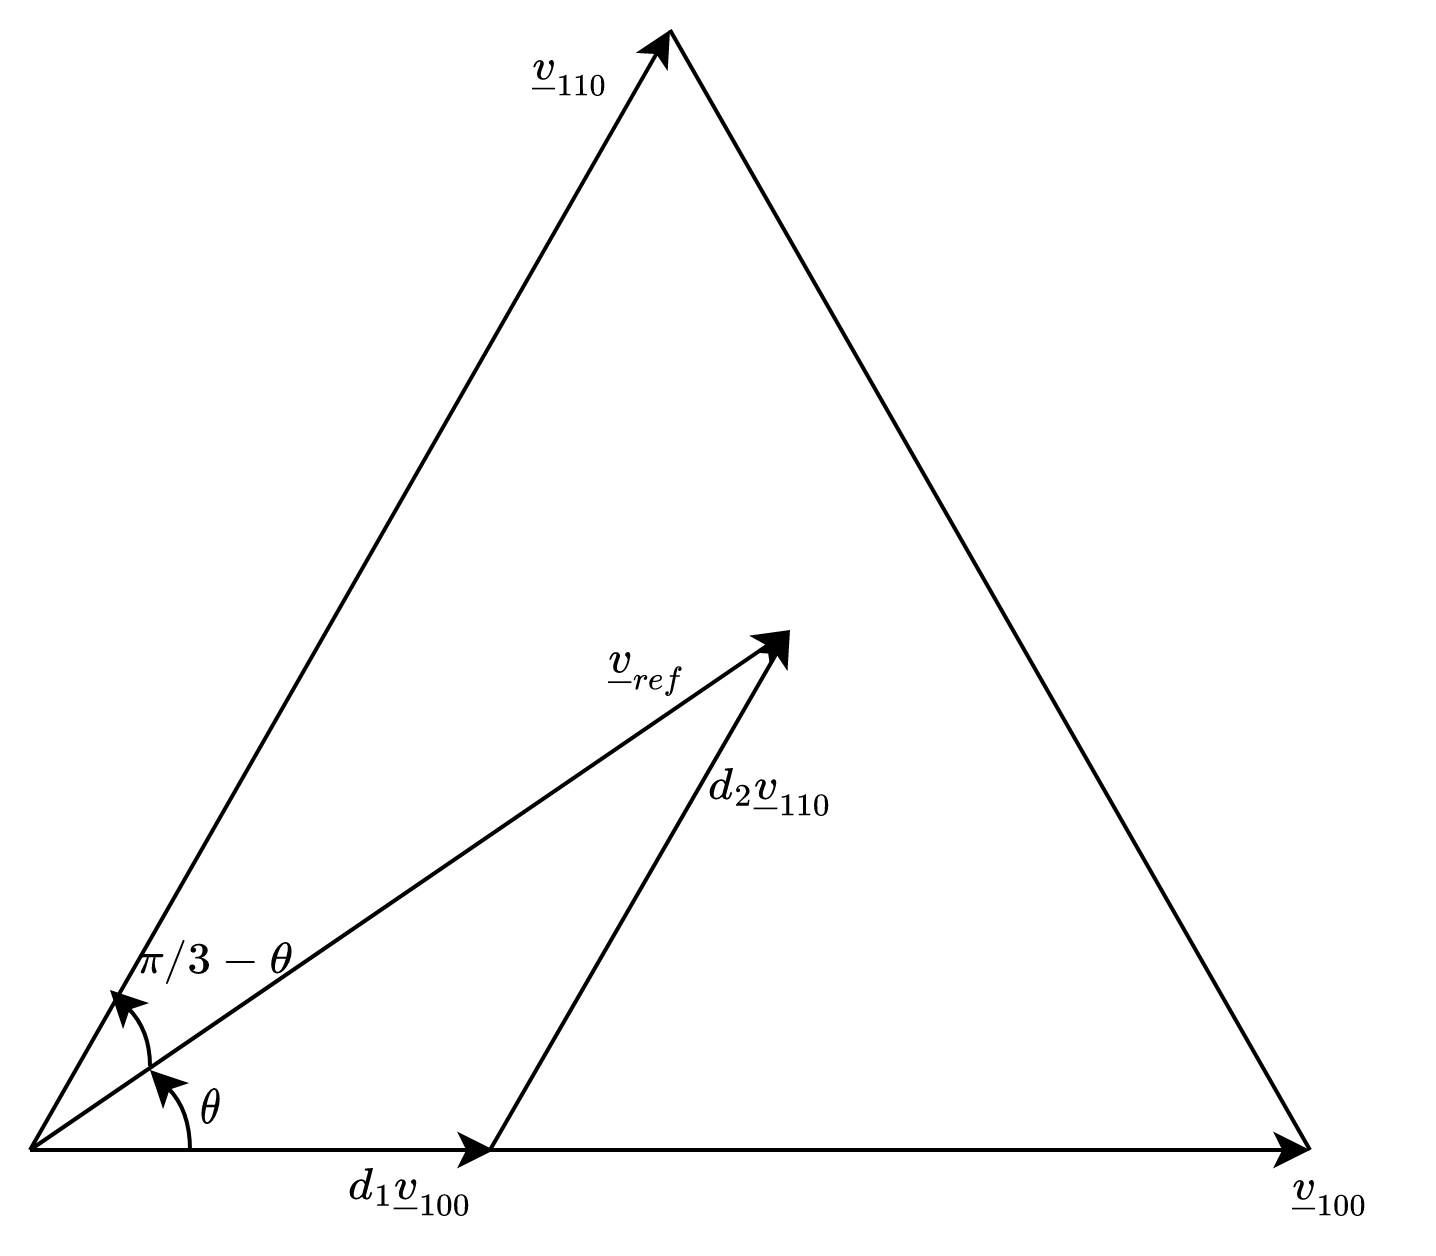
\includegraphics[width=0.75\linewidth]{images/modulation/modulation-sector} \caption{A sector of the modulation hexagon.}\label{fig:unnamed-chunk-2}
\end{figure}

The duty-cycles are calculated here, from sector 1 on the figure above.

\[
\begin{aligned}
\underline{v}_{ref} &  = d_1 \underline{v}_{100} + d_2 \underline{v}_{110}\\
 &  = d_1 \frac{2}{3} V_d  + d_2 \frac{2}{3} V_d (\frac{1}{2}+j\frac{\sqrt{3}}{2})\\
 &  = \frac{2}{3} V_d ( d_1   + d_2  (\frac{1}{2}+j\frac{\sqrt{3}}{2}))\\
 &  = \frac{2}{3} V_d ( (d_1   + d_2  \frac{1}{2})+jd_2\frac{\sqrt{3}}{2})\\
\end{aligned}
\]
Splitting into real and imaginary parts, we get from the imaginary part:

\[
\begin{aligned}
 | \underline{v}_{ref}| \sin\theta  &  = \frac{2}{3} V_d d_2 \frac{\sqrt{3}}{2}\\
\Rightarrow | \underline{v}_{ref}| \sin\theta  &  = \frac{2}{3} V_d d_2 \frac{\sqrt{3}}{2}\\
\Rightarrow d_2  &  =  \frac{|\underline{v}_{ref}|}{V_d/\sqrt{3}} \sin\theta \\
\end{aligned}
\]
And from the real part:
\[
\begin{aligned}
| \underline{v}_{ref}| \cos\theta &  = \frac{2}{3} V_d ( d_1   + d_2  \frac{1}{2})\\
\Rightarrow  d_1  &  =  \frac{3}{2} \frac{|\underline{v}_{ref}|}{V_d}   \cos\theta  - \frac{1}{2}d_2\\
\Rightarrow  d_1  &  =  \frac{\sqrt{3}}{2} \frac{|\underline{v}_{ref}|}{V_d/\sqrt{3}}   \cos\theta  - \frac{1}{2}d_2\\
\end{aligned}
\]
The modulation index is defined as \(m_i=|\underline{v}_{ref}|/(V_d/\sqrt{3})\), so the duty-cycles can be formulated as:

\[
\begin{aligned}
d_2  &  =  m_i \sin\theta \\
d_1  &  =  \frac{\sqrt{3}}{2} m_i   \cos\theta  - \frac{1}{2}d_2\\
\end{aligned}
\]
Instead of projecting on the real and imaginary axes, we can make a projection onto the axis perpendicular to \(v_{110}\):

\[
\begin{aligned}
d_1|\underline{v}_{110}| \frac{\sqrt{3}}{2}  &  =  |\underline{v}_{ref}|\sin(\frac{\pi}{3}-\theta)  \\
\Rightarrow d_1 \frac{2}{3} V_d  \frac{\sqrt{3}}{2}  &  =  |\underline{v}_{ref}|\sin(\frac{\pi}{3}-\theta)\\
\Rightarrow d_1   &  =  \frac{|\underline{v}_{ref}|}{V_d/\sqrt{3}}  \sin(\frac{\pi}{3}-\theta)\\
\Rightarrow d_1   &  =  m_i  \sin(\frac{\pi}{3}-\theta)\\
\end{aligned}
\]

This way the duty-cycles can be calculated as:
\[
\begin{aligned}
d_1   &  =  m_i  \sin(\frac{\pi}{3}-\theta)\\
d_2  &  =  m_i \sin\theta \\
\end{aligned}
\]

Furthermore, the zero-vector dutycycle is:
\[
d_0 = 1 - d_1 - d_2
\]

\hypertarget{space-vector-modulation-svm.}{%
\section{Space Vector Modulation (SVM).}\label{space-vector-modulation-svm.}}

In space vector modulation the active vectors are placed in the middle and the zero-vectors are evenly placed in the beginning and the end. An example is shown here:

\begin{figure}
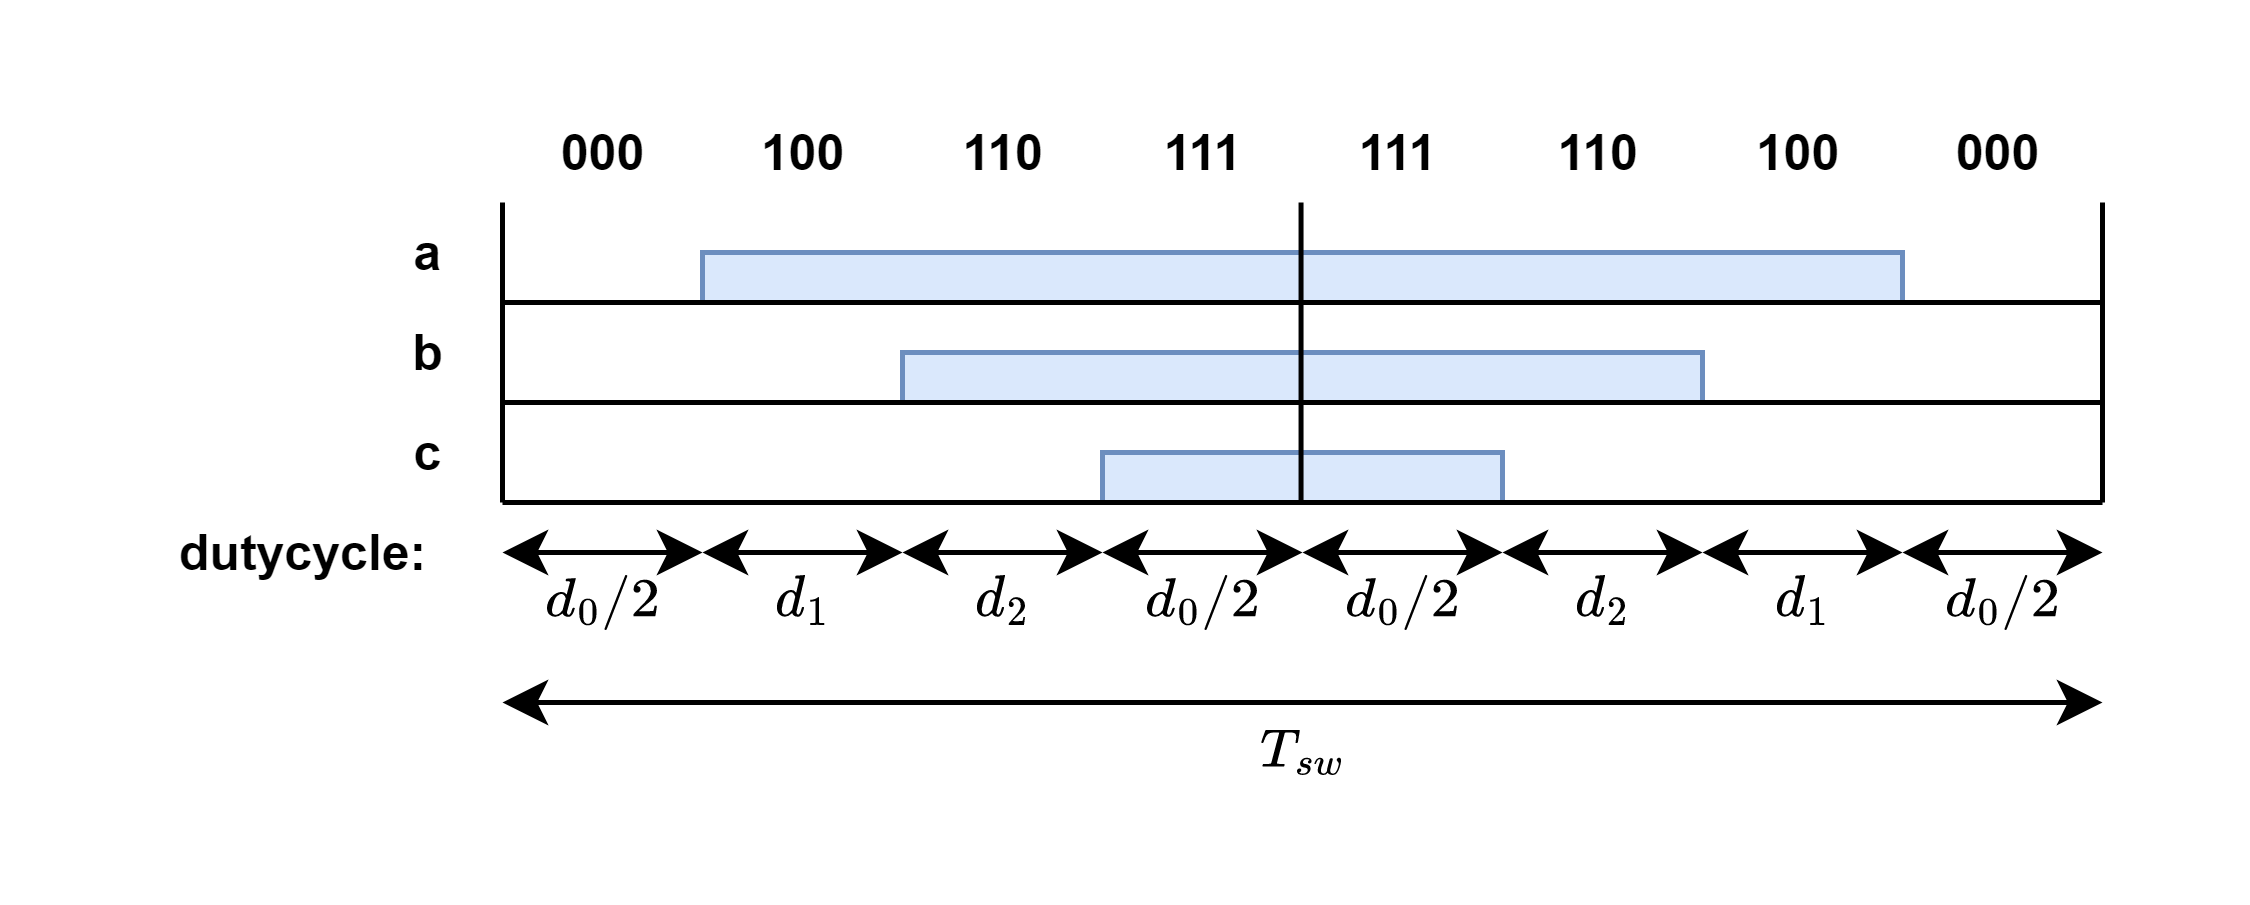
\includegraphics[width=1\linewidth]{images/modulation/switchperiod} \caption{Pwm pulses over one switching period for sector 1 with spacevector modulation.}\label{fig:unnamed-chunk-3}
\end{figure}

\begin{figure}
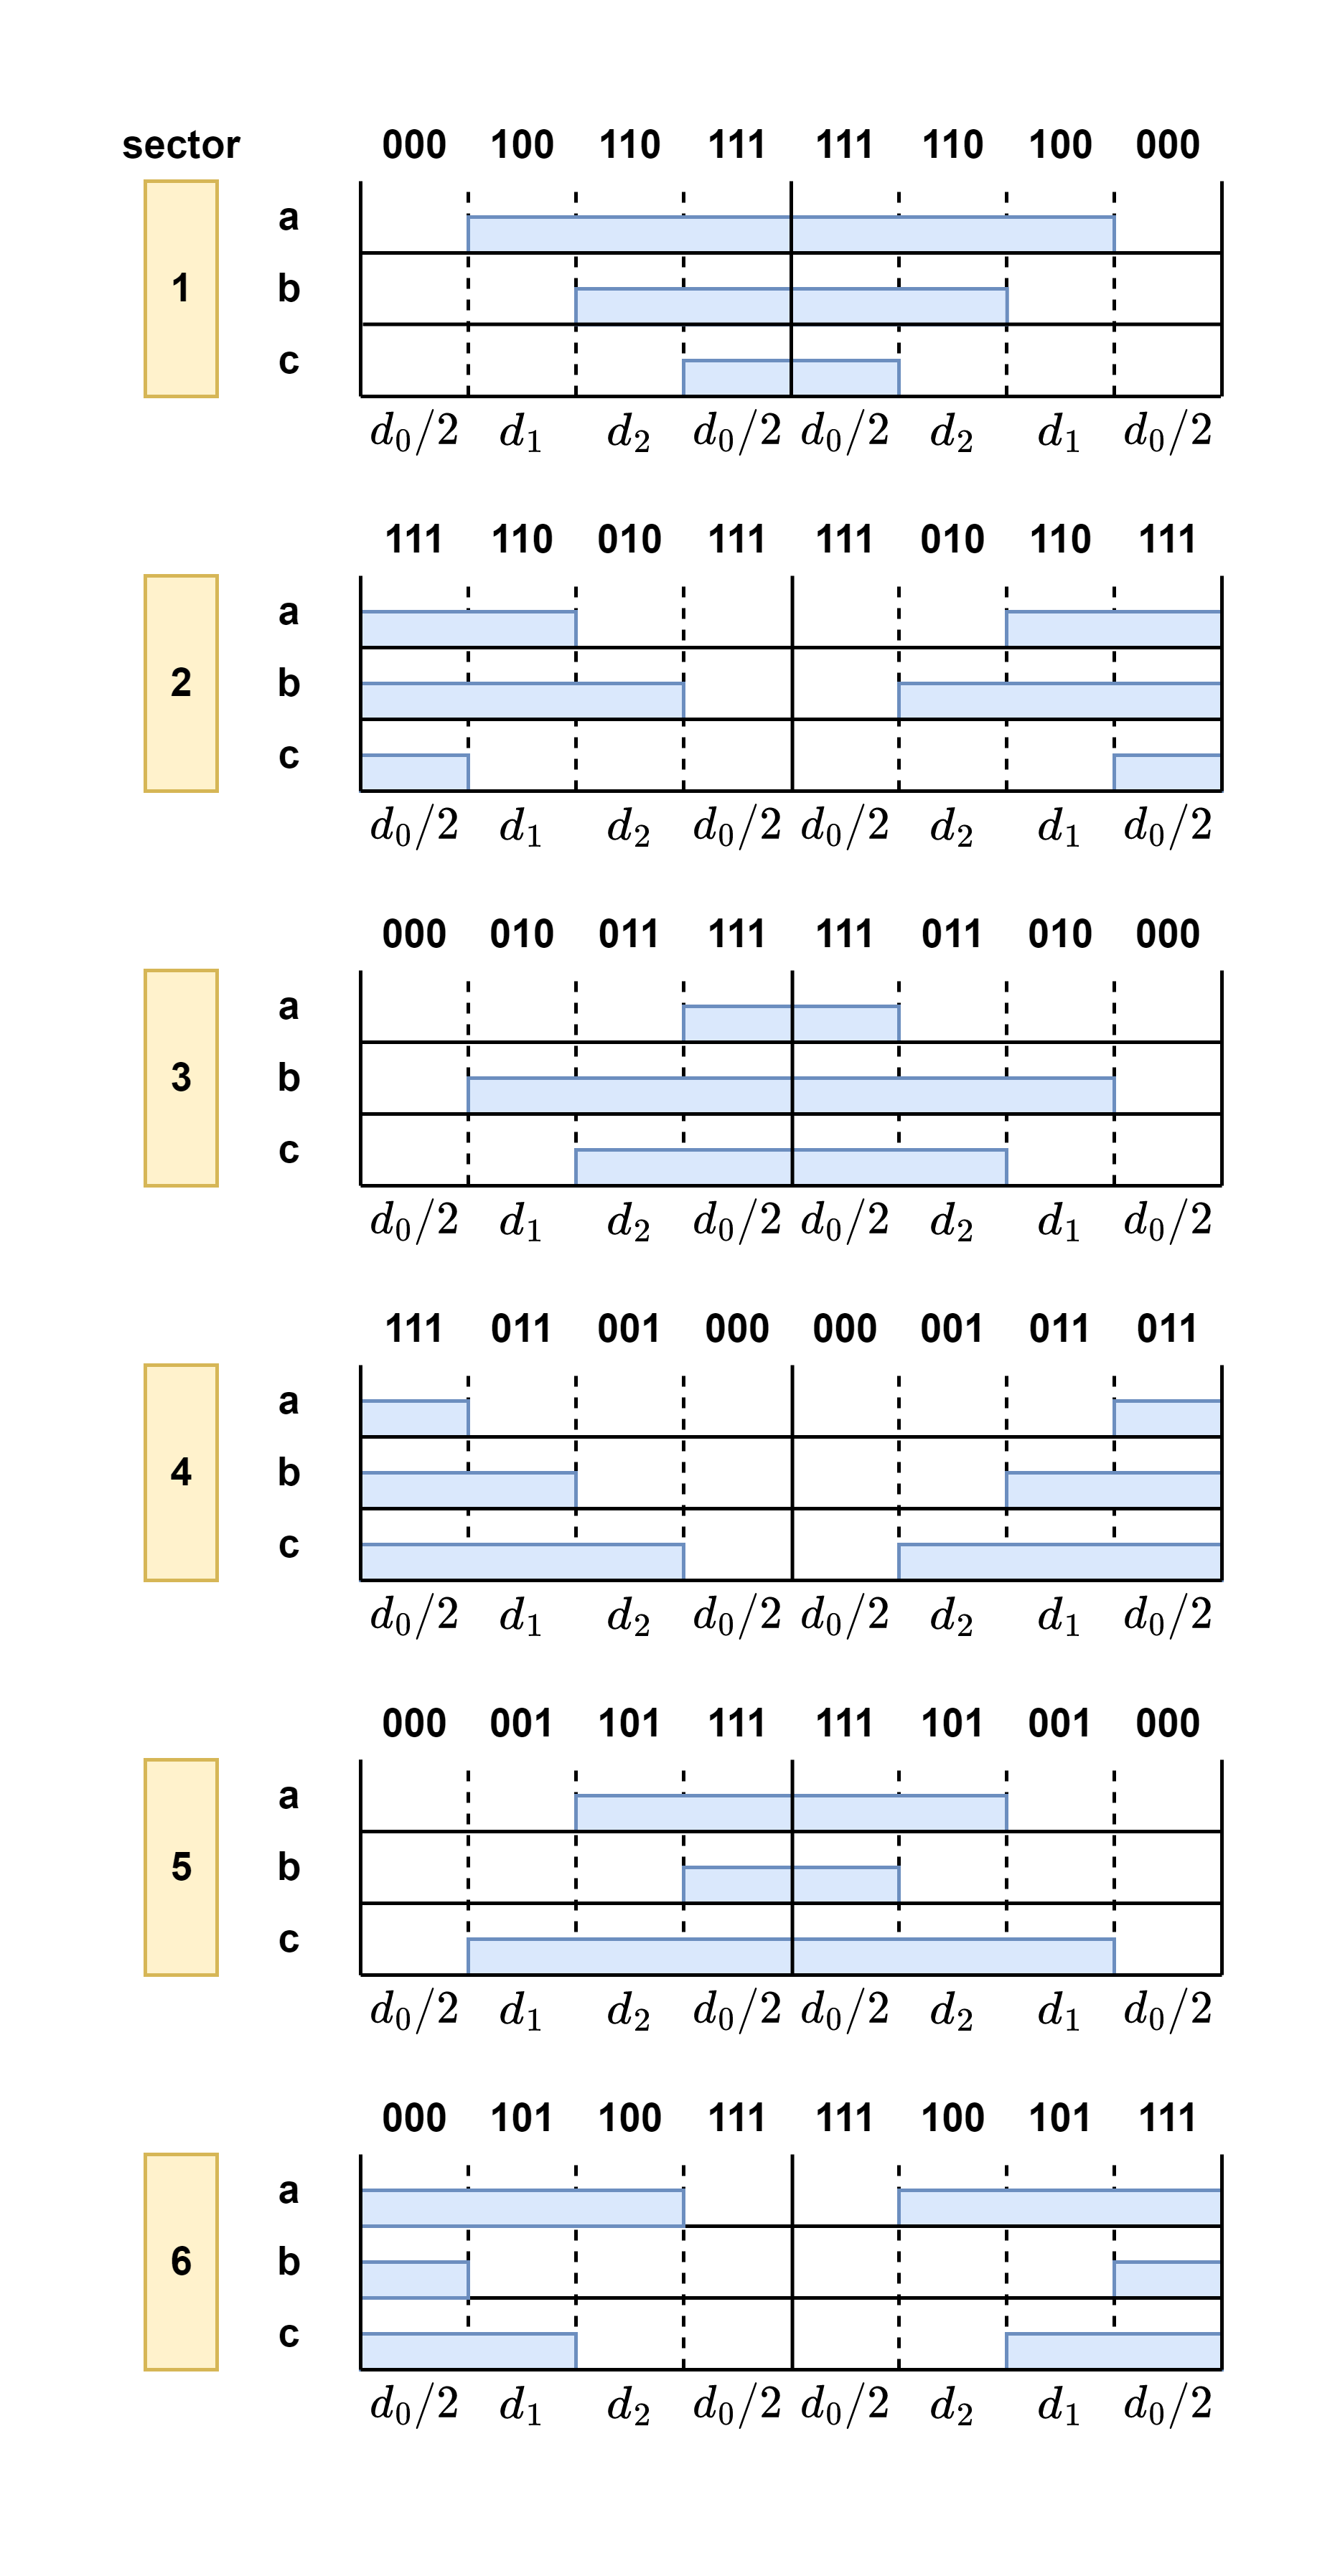
\includegraphics[width=1\linewidth]{images/modulation/svm-pulses} \caption{Spacevector modulation pulses for all six sectors.}\label{fig:unnamed-chunk-4}
\end{figure}

The duty-cycles for phases a, b and c are calculated as:

\[
\begin{aligned}
\text{sector 1}&\\
d_a  &  =  d_0/2 + d_2+d_1\\
d_b  &  =  d_0/2 + d_2\\
d_c  &  =  d_0/2\\
\text{sector 2}&\\
d_a  &  =  d_0/2 + d_1\\
d_b  &  =  d_0/2 + d_1+d_2\\
d_c  &  =  d_0/2\\
\text{sector 3}&\\
d_a  &  =  d_0/2 \\
d_b  &  =  d_0/2 + d_2+d_1\\
d_c  &  =  d_0/2 + d_2\\
\text{sector 4}&\\
d_a  &  =  d_0/2\\
d_b  &  =  d_0/2 + d_1\\
d_c  &  =  d_0/2 + d_1+d_2\\
\text{sector 5}&\\
d_a  &  =  d_0/2 + d_2\\
d_b  &  =  d_0/2\\
d_c  &  =  d_0/2 + d_2+d_1\\
\text{sector 6}&\\
d_a  &  =  d_0/2 + d_1+d_2\\
d_b  &  =  d_0/2\\
d_c  &  =  d_0/2 + d_1\\
\end{aligned}
\]

\begin{figure}
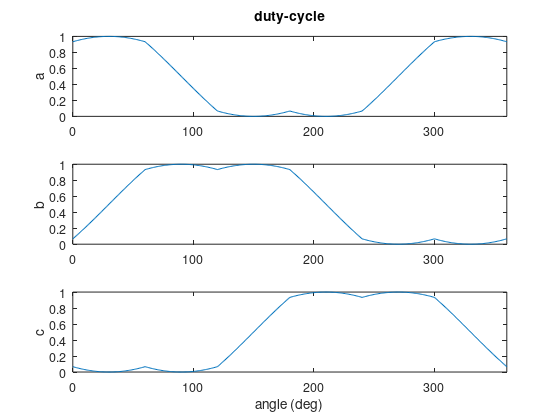
\includegraphics[width=1\linewidth]{images/modulation/svm-dutycycle} \caption{Spacevector modulation duty-cycle for phase a, b, and c, for modulation index = 1.}\label{fig:unnamed-chunk-5}
\end{figure}

\hypertarget{duty-cycle-function-expression.}{%
\section{Duty-cycle function expression.}\label{duty-cycle-function-expression.}}

The duty-cycles are reformulated for sector 1, by inserting \(d_0 = 1-d_1-d_2\) in the expression above:

\[
\begin{aligned}
d_a  &  = \frac{1}{2} (1+ d_1+d_2)\\
d_b  &  = \frac{1}{2} (1- d_1+d_2)\\
d_c  &  = \frac{1}{2} (1- d_1-d_2)\\
\end{aligned}
\]

For sector 1 we get:

\[
\begin{aligned}
d_a  &  = \frac{1}{2} (1+ d_1+d_2)\\
&  =  \frac{1}{2} (1+ (\frac{\sqrt{3}}{2} m_i   \cos\theta  - \frac{1}{2}d_2)+d_2) \\
&  =  \frac{1}{2} (1+ \frac{\sqrt{3}}{2} m_i   \cos\theta  + \frac{1}{2} m_i \sin\theta ) \\
&  =  \frac{1}{2} + \frac{1}{2} m_i( \frac{\sqrt{3}}{2}  \cos\theta  + \frac{1}{2} \sin\theta ) \\
\end{aligned}
\]

\[
\begin{aligned}
d_b  &  = \frac{1}{2} (1- d_1+d_2)\\
&  =  \frac{1}{2} (1- (\frac{\sqrt{3}}{2} m_i   \cos\theta  - \frac{1}{2}d_2)+d_2) \\
&  =  \frac{1}{2} (1- \frac{\sqrt{3}}{2} m_i   \cos\theta  + \frac{3}{2} m_i \sin\theta ) \\
&  =  \frac{1}{2} - \frac{1}{2} m_i( \frac{\sqrt{3}}{2}  \cos\theta  - \frac{3}{2} \sin\theta ) \\
\end{aligned}
\]

\[
\begin{aligned}
d_c  &  = \frac{1}{2} (1- d_1-d_2)\\
&  =  \frac{1}{2} (1- (\frac{\sqrt{3}}{2} m_i   \cos\theta  - \frac{1}{2}d_2)-d_2) \\
&  =  \frac{1}{2} (1- \frac{\sqrt{3}}{2} m_i   \cos\theta  - \frac{1}{2} m_i \sin\theta ) \\
&  =  \frac{1}{2} - \frac{1}{2} m_i( \frac{\sqrt{3}}{2}  \cos\theta  + \frac{1}{2} \sin\theta ) \\
\end{aligned}
\]

\hypertarget{calculation-of-duty-cycle-from-phase-voltage-references.}{%
\section{Calculation of duty-cycle from phase-voltage references.}\label{calculation-of-duty-cycle-from-phase-voltage-references.}}

As an alternative to calculate the duty-cycles from the space-vector, they can be calculated from the phase-voltage references directly.

\[
\begin{aligned}
d_a  & = \frac{1}{2} \left( \frac{(v_{ref,a} - v_{cm})}{V_d/2} +1 \right) = \frac{1}{2} +\frac{1}{V_d}  (v_{ref,a} - v_{cm}) \\
d_b  & = \frac{1}{2} \left( \frac{(v_{ref,b} - v_{cm})}{V_d/2} +1 \right) = \frac{1}{2} +\frac{1}{V_d}  (v_{ref,b} - v_{cm}) \\
d_c  & = \frac{1}{2} \left( \frac{(v_{ref,c} - v_{cm})}{V_d/2} +1 \right) = \frac{1}{2} +\frac{1}{V_d}  (v_{ref,c} - v_{cm}) \\
\end{aligned}
\]
where:
\(v_{ref,a}\): reference voltage, phase a, phase-zero voltage.\\
\(v_{ref,b}\): reference voltage, phase b, phase-zero voltage.\\
\(v_{ref,c}\): reference voltage, phase c, phase-zero voltage.\\
\(v_{cm}\): common-mode voltage.\\
\(V_d\): Dc-link voltage.\\
\(d_a\): duty-cycle, phase a, range 0-1.\\
\(d_b\): duty-cycle, phase b, range 0-1.\\
\(d_c\): duty-cycle, phase c, range 0-1.

The common-mode voltage can have any shape, and space-vector modulation is achieved with this common-mode signal, which is the mean value of the max and min phase voltage references:

\[
\begin{aligned}
v_{cm}  &  = \frac{1}{2}  ( \text{min}(v_a, v_b, v_c) + \text{max}(v_a, v_b, v_c))\\
\end{aligned}
\]

We can now show that this does give the same result as the previously derived expressions. As an example of this, we calculate the duty-cycle for phase a in sector 1. From the figure below we can see that phase a is the highest and phase c the lowest.

\begin{figure}
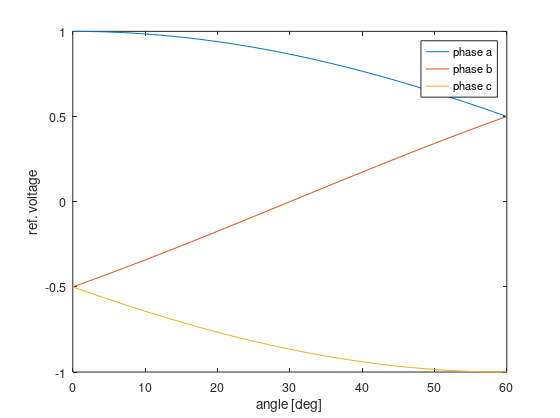
\includegraphics[width=0.75\linewidth]{images/modulation/phase-ref-voltages-abc} \caption{Voltage references for phase a, b, and c.}\label{fig:unnamed-chunk-6}
\end{figure}

\[
\begin{aligned}
v_a-v_{cm}  & = |\underline{v}_{ref}| \left( \cos{\theta} - \frac{1}{2}(\cos{\theta}  + \cos{(\theta - 4\pi/3)})  \right)\\
& = |\underline{v}_{ref}| \left( \cos{\theta} - \frac{1}{2}(\cos{\theta}  + \cos{(4\pi/3)}\cos{\theta}+\sin{( 4\pi/3)}\sin{\theta})  \right)\\
& = |\underline{v}_{ref}| \left( \cos{\theta} - \frac{1}{2}(\cos{\theta}  - \frac{1}{2}\cos{\theta} - \frac{\sqrt{3}}{2}\sin{\theta})  \right)\\
& = |\underline{v}_{ref}| ( \frac{3}{4} \cos{\theta}  + \frac{\sqrt{3}}{4}\sin{\theta}  )\\
\end{aligned}
\]

Now the duty-cycle can be derived as:

\[
\begin{aligned}
d_a  & = \frac{1}{2} +\frac{1}{V_d}  (v_{ref,a} - v_{cm}) \\
  & = \frac{1}{2} +\frac{1}{V_d}  |\underline{v}_{ref}| ( \frac{3}{4} \cos{\theta}  + \frac{\sqrt{3}}{4}\sin{\theta}  ) \\
  & = \frac{1}{2} + \frac{1}{2} \frac{|\underline{v}_{ref}|}{V_d/\sqrt{3}} ( \frac{\sqrt{3}}{2} \cos{\theta}  + \frac{1}{2}\sin{\theta}  ) \\
& = \frac{1}{2} +  \frac{1}{2} m_i  ( \frac{\sqrt{3}}{2} \cos{\theta}  + \frac{1}{2}\sin{\theta}  ) \\
\end{aligned}
\]
In the similar way, the expression can be derived for the other phases and other sectors.

\hypertarget{induction-machine}{%
\chapter{Induction Machine}\label{induction-machine}}

\hypertarget{nomenclature}{%
\section{Nomenclature}\label{nomenclature}}

\(\underline{v}_s\): Stator voltage vector.\\
\(\underline{v}_r\): Rotor voltage vector.\\
\(R_s\): Stator resistance.\\
\(R_r\): Rotor resistance.\\
\(\underline{\psi}_s\): Stator flux linkage.\\
\(\underline{\psi}_r\): Rotor flux linkage.\\
\(\omega_c\): Angular frequency of reference frame.\\
\(\omega_m\): Angular frequency of shaft in electrical frame, i.e compensated for pole-pairs.\\
\(L_m\): Magnetizing inductance.\\
\(L_m\): Magnetizing inductance.\\
\(L_{s\sigma}\): Stator leakage inductance.\\
\(L_{r\sigma}\): Rotor leakage inductance.\\
\(L_s\): Stator inductance. \(L_s = L_m + L_{s\sigma}\)\\
\(L_r\): Rotor inductance. \(L_r = L_m + L_{r\sigma}\)\\
\(1-\frac{L^2_m}{L_sL_r}\): total leakage coefficient.\\
\(ms\): magnetizing-stator super/subscript, stator flux oriented reference frame.\\
\(mr\): magnetizing-rotor super/subscript, rotor flux oriented reference frame.\\
\(g\): super/subscript, general reference frame.\\
\(\tau_{em}\): electro-magnetic torque.\\
\(N_{pp}\): pole-pair number.\\

\hypertarget{introduction}{%
\section{Introduction}\label{introduction}}

The general dynamic machine model in a rotating reference frame is first presented. Then it is shown how it is derived from the stationary reference frame equations.

The rotor-flux oriented reference frame equations are derived. This particular model is often used for vector-oriented control from the stator side.

\hypertarget{general-machine-model}{%
\section{General Machine Model}\label{general-machine-model}}

In short, the dynamics of the inductions machine is described by this dynamic vector model:

\[
\begin{aligned}
\underline{v}_s & = R_s \underline{i}_s + \frac{d\underline{\psi}_s}{dt} + j \omega_g \underline{\psi}_s  \\
\underline{v}_r & = R_r \underline{i}_r + \frac{d\underline{\psi}_r}{dt} + j (\omega_g-\omega_m) \underline{\psi}_r \\
\underline{\psi}_s & = L_s \underline{i}_s + L_m \underline{i}_r\\
\underline{\psi}_r & = L_m \underline{i}_s + L_r \underline{i}_r\\
\tau_{em} &= - \frac{3}{2}N_{pp}L_m(\underline{i}_s  \times \underline{i}_r)
\end{aligned}
\label{eq:genDqMdl}
\]

This model is with motor sign, in a general reference frame g.

In this notation all quantities are seen from the same side of the machine. So, when seen from the stator, the rotor current in not the physical rotor current, but the rotor current as seen from the stator. The same goes for flux, voltage and impedance. So we don't use a apostrophe to note that rotor quantities are transferred values, as it is sometimes done.

This is not a special issue for a squirrel cage machine, where we do not have easy access to rotor quantities anyway, by we practically always look the the machine from the stator. But for the doubly-fed induction machine, where we have access to both the stator and the rotor circuit, special care must be taken to transfer values from one side to the other.

\hypertarget{stator-equation}{%
\subsection{Stator Equation}\label{stator-equation}}

The stator equation in the stator reference frame is:
\[
\begin{aligned}
\underline{v}_s & = R_s \underline{i}_s + \frac{d\underline{\psi}_s}{dt}  \\
\end{aligned}
\label{eq:statorVoltStat}
\]
We want to express this in a general reference frame, where \(\rho_s\) is the angle from the stator fixed frame to the general reference frame. With the superscripts denoting the reference frames, s for stator, g for general, we can write:
\[
\begin{aligned}
\underline{v}^s_s & = \underline{v}^g_s e^{j\rho_s} \\
\underline{i}^s_s & = \underline{i}^g_s e^{j\rho_s} \\
\underline{\psi}^s_s & = \underline{\psi}^g_s e^{j\rho_s} \\
\frac{d\underline{\psi}^s_s}{dt}  & = \frac{d (\underline{\psi}^g_s e^{j\rho_s} )}{dt}  = 
\frac{d\underline{\psi}^g_s}{dt}  e^{j\rho_s} + \underline{\psi}^g_s j \omega_g e^{j\rho_s},
\omega_g = \frac{d\rho_s}{dt} \\
\end{aligned}
\label{eq:statorVoltStat1}
\]
By inserting these in the stator equation above, we get:

\[
\begin{aligned}
\underline{v}^s_s & = R_s \underline{i}^s_s + \frac{d\underline{\psi}^s_s}{dt}  \\
\underline{v}^g_s e^{j\rho_s} & = R_s \underline{i}^g_s e^{j\rho_s} + \frac{d\underline{\psi}^g_s}{dt}  e^{j\rho_s} + \underline{\psi}^g_s j \omega_g e^{j\rho_s}  \\
\underline{v}^g_s  & = R_s \underline{i}^g_s  + \frac{d\underline{\psi}^g_s}{dt}   + j\underline{\psi}^g_s  \omega_g   \\
\end{aligned}
\label{eq:statorVoltStat2}
\]
this is the general stator equation, see \eqref{eq:genDqMdl}

\hypertarget{rotor-equation}{%
\subsection{Rotor Equation}\label{rotor-equation}}

The rotor equation in the rotor reference frame is:
\[
\begin{aligned}
\underline{v}_r & = R_r \underline{i}_r + \frac{d\underline{\psi}_r}{dt}  \\
\end{aligned}
\label{eq:rotorVoltStat1}
\]
We want to express this in a general reference frame, where \(\rho_r\) is the angle from the rotor fixed frame to the general reference frame. With the superscripts denoting the reference frames, r for rotor, g for general, we can write:
\[
\begin{aligned}
\underline{v}^r_r & = \underline{v}^g_r e^{j\rho_r} \\
\underline{i}^r_r & = \underline{i}^g_r e^{j\rho_r} \\
\underline{\psi}^r_r & = \underline{\psi}^g_r e^{j\rho_r} \\
\frac{d\underline{\psi}^r_r}{dt}  & = \frac{d (\underline{\psi}^g_r e^{j\rho_r} )}{dt}  = 
\frac{d\underline{\psi}^g_r}{dt}  e^{j\rho_r} + \underline{\psi}^g_r j (\omega_g-\omega_r) e^{j\rho_r},
\omega_g-\omega_r = \frac{d\rho_r}{dt} \\
\end{aligned}
\label{eq:rotorVoltStat2}
\]
By inserting these in the rotor equation above, we get:

\[
\begin{aligned}
\underline{v}^r_r & = R_r \underline{i}^r_r + \frac{d\underline{\psi}^r_r}{dt}  \\
\underline{v}^g_r e^{j\rho_r} & = R_r \underline{i}^g_r e^{j\rho_r} + \frac{d\underline{\psi}^g_r}{dt}  e^{j\rho_r} + \underline{\psi}^g_r j (\omega_g-\omega_r) e^{j\rho_r}  \\
\underline{v}^g_r  & = R_r \underline{i}^g_r  + \frac{d\underline{\psi}^g_r}{dt}   + j \underline{\psi}^g_r  (\omega_g-\omega_r)  \\
\end{aligned}
\label{eq:rotorVoltStat3}
\]

this is the general rotor equation, see \eqref{eq:genDqMdl}

\hypertarget{torque-equations}{%
\subsection{Torque Equations}\label{torque-equations}}

The electrical torque can be expressed in terms of cross-product as:
\[
\begin{aligned}
\tau_{em} &= - \frac{3}{2}N_{pp}L_m(\underline{i}_s  \times \underline{i}_r) \\
&= - \frac{3}{2}N_{pp}L_m(i_{sd}i_{rq} -  i_{sq}i_{rd}) \\
&= - \frac{3}{2}N_{pp}L_m Im(\underline{i}^*_s  \cdot \underline{i}_r) \\
\end{aligned}
\label{eq:torque1}
\]

The last line contains the imaginary part of the complex-conjugate stator current and the rotor current.
The torque can be calculated in various other ways, to be elaborated.

\hypertarget{rotor-flux-oriented-model}{%
\section{Rotor-flux Oriented Model}\label{rotor-flux-oriented-model}}

For the rotor-flux oriented Model, the d-axis is oriented with the rotor flux, so the rotor-flux has no q-axis component.

The rotor magnetizing current \(\underline{i}_{mr}\) is defined as:

\[
\underline{i}_{mr} = \frac{\underline{\psi}_r}{L_m}= \frac{L_m\underline{i}_s+L_r\underline{i}_r}{L_m}
= \underline{i}_s+ \frac{L_r}{L_m}\underline{i}_r
\label{eq:rotorFluxFlux1}
\]

\[
\underline{i}_r = \frac{L_m}{L_r} (\underline{i}_{mr} -  \underline{i}_s)
\label{eq:rotorFluxFlux2}
\]
The stator flux can be calculated as:
\[
\begin{aligned}
\underline{\psi}_s
& = L_s\underline{i}_s + L_m\underline{i}_r \\
& = L_s\underline{i}_s + L_m \frac{L_m}{L_r} (\underline{i}_{mr} -  \underline{i}_s) \\
& =  \frac{L^2_m}{L_r}\underline{i}_{mr}  + L_s\underline{i}_s - \frac{L^2_m}{L_r}  \underline{i}_s \\
& =  \frac{L^2_m}{L_r}\underline{i}_{mr}  + L_s(1 - \frac{L^2_m}{L_s L_r} ) \underline{i}_s \\
& =  \frac{L^2_m}{L_r}\underline{i}_{mr}  + \sigma L_s \underline{i}_s  \\
\end{aligned}
\label{eq:rotorFluxFlux3}
\]

the leakage constant being defined as: \(\sigma=1 - \frac{L^2_m}{L_s L_r}\)

\hypertarget{rotor-voltage-equation-rotor-flux-oriented}{%
\subsection{Rotor voltage equation (rotor-flux oriented)}\label{rotor-voltage-equation-rotor-flux-oriented}}

\[
\begin{aligned}
\underline{v}^{mr}_r  & = R_r \underline{i}^{mr}_r  + \frac{d\underline{\psi}^{mr}_r}{dt} + j (\omega_{mr}-\omega_r) \underline{\psi}^{mr}_r    \\
& = R_r  \frac{L_m}{L_r} (\underline{i}_{mr} -  \underline{i}_s) + \frac{d ( L_m \underline{i}_{mr}) }{dt} + j (\omega_{mr}-\omega_r) L_m \underline{i}_{mr} \\
& =  -\underline{i}_s R_r  \frac{L_m}{L_r}  + L_m \frac{d  \underline{i}_{mr} }{dt} + R_r  \frac{L_m}{L_r} \underline{i}_{mr}  + j (\omega_{mr}-\omega_r) L_m \underline{i}_{mr} \\
\end{aligned}
\label{eq:rotorFluxRotVolt1}
\]

\[
\begin{aligned}
\frac{L_r}{R_r L_m} \underline{v}^{mr}_r  & =  -\underline{i}^{mr}_s   + \frac{L_r}{R_r} \frac{d  \underline{i}_{mr} }{dt} + \underline{i}_{mr}  + j (\omega_{mr}-\omega_r) \frac{L_r}{R_r} \underline{i}_{mr} \\
\frac{L_r}{R_r L_m} \underline{v}^{mr}_r +\underline{i}^{mr}_s  & =  \frac{L_r}{R_r} \frac{d  \underline{i}_{mr} }{dt} + \underline{i}_{mr}  + j (\omega_{mr}-\omega_r) \frac{L_r}{R_r} \underline{i}_{mr} \\
\end{aligned}
\label{eq:rotorFluxRotVolt2}
\]

\[
\begin{aligned}
\frac{L_r}{R_r L_m} v_{rd} +i_{sd}  & =  \frac{L_r}{R_r} \frac{d  i_{mr} }{dt} + i_{mr} \\
\frac{L_r}{R_r L_m} v_{rq} +i_{sq}  & =  (\omega_{mr}-\omega_r) \frac{L_r}{R_r} i_{mr} \\
\end{aligned}
\label{eq:rotorFluxRotVolt3}
\]

\hypertarget{stator-voltage-equation-rotor-flux-oriented}{%
\subsection{Stator voltage equation (rotor-flux oriented)}\label{stator-voltage-equation-rotor-flux-oriented}}

\[
\begin{aligned}
\underline{v}^{mr}_s & = R_s \underline{i}^{mr}_s  + \frac{d\underline{\psi}^{mr}_s}{dt}   + j\omega_{mr}  \underline{\psi}^{mr}_s  \\
 & = R_s \underline{i}^{mr}_s  + \frac{d}{dt}(\frac{L^2_m}{L_r}\underline{i}^{mr}_{mr}  + \sigma L_s \underline{i}_s)   + j\omega_{mr}  (\frac{L^2_m}{L_r}\underline{i}^{mr}_{mr}  + \sigma L_s \underline{i}_s)  \\
 & = R_s \underline{i}^{mr}_s  + \frac{d}{dt}( (1-\sigma)L_s i_{mr}  + \sigma L_s \underline{i}_s)   + j\omega_{mr}  ((1-\sigma)L_s i_{mr}  + \sigma L_s \underline{i}_s)  \\
\end{aligned}
\label{eq:rotorFluxStaVolt1}
\]

\[
\begin{aligned}
v_{sd} & = R_s i_{sd}  + \sigma L_s \frac{d i_{sd}}{dt} + (1-\sigma)L_s \frac{d i_{mr}}{dt} - \omega_{mr}     \sigma L_s i_{sq}  \\
v_{sq} & = R_s i_{sq}  + \sigma L_s \frac{d i_{sq}}{dt} + \omega_{mr}  ((1-\sigma)L_s i_{mr}  + \sigma L_s i_{sd})  \\
\end{aligned}
\label{eq:rotorFluxStaVolt2}
\]

\hypertarget{torque-equation-rotor-flux-oriented}{%
\subsection{Torque equation (rotor-flux oriented)}\label{torque-equation-rotor-flux-oriented}}

The electrical torque can be expressed in terms of cross-product as:
\[
\begin{aligned}
\tau_{em} &= - \frac{3}{2}N_{pp}L_m(i_{sd}i_{rq} -  i_{sq}i_{rd}) \\
&=  \frac{3}{2}N_{pp}L_m i_{rd}  i_{sq} \\
\end{aligned}
\label{eq:rotorFluxTorque1}
\]

\hypertarget{pm-machine}{%
\chapter{PM Machine}\label{pm-machine}}

\hypertarget{nomenclature-1}{%
\section{Nomenclature}\label{nomenclature-1}}

\(R_s\): Stator resistance.\\
\(\psi_{pm}\): Permament magnet flux linkage.\\
\(\omega_m\): Angular frequency of shaft in electrical frame, i.e compensated for pole-pairs.\\
\(L_d\): d-axis inductance.\\
\(L_q\): q-axis inductance.\\
\(\tau_{em}\): Electro-magnetic torque.\\
\(N_{pp}\): Pole-pair number.

\hypertarget{machine-equations}{%
\section{Machine Equations}\label{machine-equations}}

\[
\begin{aligned}
v_d & = R_s i_d + L_d\frac{di_d}{dt} - j \omega_m L_q i_q  \\
v_q & = R_s i_q + L_q\frac{di_q}{dt} + j \omega_m (L_d i_d + \psi_{pm})  \\
\tau_{em} & =  (\psi_{pm} + (L_d-L_q) i_d)i_q  \\
\end{aligned}
\label{eq:pmsmMdl1}
\]

\hypertarget{maximum-torque-per-ampere-mtpa}{%
\section{Maximum Torque Per Ampere (MTPA)}\label{maximum-torque-per-ampere-mtpa}}

MTPA is a commonly used control strategy by which the current is controlled to produce the maximum torque for at given current amplitude. It is shown here how the control equations are derived. This is done from the torque equation:

\[
\begin{aligned}
T_{em} & =  (\psi_{pm} + (L_d-L_q) i_d)i_q  \\
\end{aligned}
\label{eq:mtpa1}
\]
The current amplitude is:
\[
|\underline{i}| = \sqrt{i^2_d + i^2_q} \Rightarrow  i_q =  (|\underline{i}|^2 - i^2_d)^{1/2} 
\label{eq:mtpa2}
\]
Inserting this in the torque equations, we get:

\[
\begin{aligned}
T_{em} & =  (\psi_{pm} + (L_d-L_q) i_d)(|\underline{i}|^2 - i^2_d)^{1/2}  \\
 & =  \psi_{pm}(|\underline{i}|^2 - i^2_d)^{1/2} + (L_d-L_q) i_d(|\underline{i}|^2 - i^2_d)^{1/2}  \\
\end{aligned}
\label{eq:mtpa3}
\]
This equation describes, for for at given current amplitude, how the torque varies as a function of \(i_d\). By differentiating, we can find the \(i_d\), which gives the maximum torque for the given current amplitude \(|\underline{i}|\).

\[
\begin{aligned}
\frac{\partial T_{em}}{\partial i_d} & =  \psi_{pm}\frac{1}{2} (|\underline{i}|^2 - i^2_d)^{-1/2} (-2i_d) + 
(L_d-L_q) \left(  (|\underline{i}|^2 - i^2_d)^{1/2}   + i_d \frac{1}{2} (|\underline{i}|^2 - i^2_d)^{-1/2} (-2i_d)  \right)  \\
 & =  -\psi_{pm} i_d (|\underline{i}|^2 - i^2_d)^{-1/2}  + 
(L_d-L_q) \left(  (|\underline{i}|^2 - i^2_d)^{1/2}   - i_d^2  (|\underline{i}|^2 - i^2_d)^{-1/2}   \right)  \\
\end{aligned}
\label{eq:mtpa3}
\]
We can now set the differential equal to zero:

\[
\begin{aligned}
\frac{\partial T_{em}}{\partial i_d} & =  0  \\
-\psi_{pm} i_d (|\underline{i}|^2 - i^2_d)^{-1/2}  + (L_d-L_q) \left(  (|\underline{i}|^2 - i^2_d)^{1/2}   - i_d^2  (|\underline{i}|^2 - i^2_d)^{-1/2}   \right) & = 0 \\
-\psi_{pm} i_d   + (L_d-L_q) \left(  |\underline{i}|^2 - i^2_d   - i_d ^2    \right) & = 0 \\
-\psi_{pm} i_d   + (L_d-L_q) (  |\underline{i}|^2 - 2i^2_d     ) & = 0 \\
 2 (L_d-L_q)i^2_d  +\psi_{pm} i_d   - (L_d-L_q)  |\underline{i}|^2  & = 0 \\
\end{aligned}
\label{eq:mtpa4}
\]
The MTPA d-current is now given as:

\[
\begin{aligned}
i_d &= \frac{-\psi_{pm} - \sqrt{\psi_{pm}^2 - 8 (L_d-L_q)^2 |\underline{i}|^2}}{4 (L_d-L_q)} \\
&= \frac{-\psi_{pm} }{4 (L_d-L_q)} -   \sqrt{\frac{\psi_{pm}^2}{16 (L_d-L_q)^2} - \frac{1}{2} |\underline{i}|^2}\\
\end{aligned}
\label{eq:mtpa5}
\]
And and q-current is calculated as:

\[
i_q = \sqrt{|\underline{i}|^2 - i^2_d }
\label{eq:mtpa6}
\]

\bibliography{book.bib,packages.bib}

\end{document}
